\documentclass[
 reprint,
 amsmath,amssymb,
 aps,
]{revtex4-1}

\usepackage{graphicx}  
\usepackage{epstopdf}
\usepackage{dcolumn}
\usepackage{bm}	
\usepackage{amsmath}			
\usepackage{amsfonts}			
\usepackage{amssymb}			
\usepackage{latexsym}		
\usepackage{color}
\usepackage{ stmaryrd }
\begin{document}

\title{Impact of Forward stimulated Brillouin scattering on the propagation of a nanosecond-class and energetic laser pulse}
\author{C. Ruyer}\email{charles.ruyer@cea.fr}
\author{A. Debayle}
\author{P. Loiseau}
\author{M. Casanova}
\author{P. E. Masson-Laborde}
\affiliation{CEA, DAM, DIF, F-91297 Arpajon, France}

\begin{abstract}
\end{abstract}

\maketitle

\section{Introduction}

\section{Paraxial propagation of an RPP beam in  driven acoustic turbulence}
\subsection{Pump wave and diffusion of  laser fields}
Following the developments of Refs. \cite[]{phd-Grech,PRL_Grech_2009}, we start by an electric field with a main propagation direction lying on the $x$-axis, a broad transverse spatial spectrum and two frequencies, $\omega_p$ and $\omega_d$ for the pump and diffused wave  respectively.  Note that the vectors are noted in bold symbols. Introducing, $D=1$ or $2$, the number of transverse direction, we assume that the electric field in real space that depends on space and time, $\mathbf{r}$  and $t$ respectively, reads
\begin{align}
E(\mathbf{r},t)= \Re \Big[ \int \frac{d^Dk_p}{(2\pi)^D} E_p (\mathbf{k}_p,t) e^{i \mathbf{k}_p \cdot \mathbf{r}_\perp} \nonumber \\
+\int \frac{d^Dk_d}{(2\pi)^D} E_d (\mathbf{k}_d,t) e^{i \mathbf{k}_d \cdot \mathbf{r}_\perp -i (\omega_d - \omega_p)t}   \Big] \, ,
\end{align}
where the subscript $\perp$ designate the transverse direction ($y,z$ and $y$ in three and two dimension respectively)  components and $\Re$  ($\Im$) the real (imaginary) part of a complex. Note that electric field, as written above,  has already been enveloped in time and space around $\omega_p$ and $k_0$ so that the physical one should be multiplied  by $\exp(k_0 x-i\omega_p t)$.

In the transverse Fourier space, dropping the dependence in time and $x$ for simplicity and with $\omega_s=\omega_d - \omega_p$,
\begin{align}
E(\mathbf{k}) =     E_p(\mathbf{k})
+  E_d(\mathbf{k}) e^{ -i \omega_s t}   \, .
\end{align} 
Using $I(k)=c\epsilon_0 \int E(k_p) E(k-k_p) dk_p$, we may split the total intensity in a pump intensity $I_p$ and diffused one $I_d$ verifying to leading order in $E_d$, \emph{i.e.} for $\vert E_d\vert \ll \vert E_p \vert$, 
\begin{align}
I(\mathbf{k}) &=I_p(\mathbf{k})+I_d(\mathbf{k})\, , \label{eq:itot}\\
I_p(\mathbf{k}_p) &=   \frac{c\epsilon_0}{2} \int E_p(\mathbf{k}) E_p^\star(\mathbf{k}_p-\mathbf{k}) d^Dk \, , \label{eq:ip} \\
I_d(\mathbf{k}_d) &\simeq   c\epsilon_0  \Re \int E_p(\mathbf{k}) E_d^\star(\mathbf{k}_d-\mathbf{k})e^{i\omega_s t } d^Dk \, , \label{eq:id}
\end{align}
with $\epsilon_0$ and  $c$, the electric permittivity and speed of light in vacuum.
In this study we will only consider wavevectors cloth to the initial
propagation direction ($x$) and note $\mathbf{k}_{p/d}=k_0\hat{\mathbf{x}} +k_{p/d,\perp}\hat{\mathbf{r}_\perp}  $ where $\hat{\mathbf{x}}$ and $\hat{\mathbf{r}_\perp}$ are unity vectors in the $x$ and transverse directions respectively. Hence, $\omega_p^2 = \omega_{pe}^2+ \mathbf{k}_p^2c^2$ and $\omega_d^2 = \omega_{pe}^2+\mathbf{k}_d^2c^2$ where $\omega_{ps}$ is the $s$-species plasma frequency and the susbscripts $e,i$ corresponds the the electrons and ions respectively.

Hence, for a pump  diffusion that occurs close to the $x$-axis,  \emph{i.e.}  $\vert \mathbf{k}_p -\mathbf{k}_d\vert \ll k_0$ and we may write to leading order the plasma wave frequency frequency and wavevector,
\begin{align}
\omega_s=\omega_p-\omega_d&= -(\mathbf{k}_s^2 c^2-2\mathbf{k}_p\cdot\mathbf{k}_s c^2)/2\omega_0
\, , \nonumber\\
\mathbf{k}_s& = \mathbf{k}_p-\mathbf{k}_d\, ,
\end{align}
where $\omega_0^2= \omega_{pe}^2+ k_0^2c^2$.
Hereafter, we will assume that the plasma wave remain mainly transverse to the pump so that $\mathbf{k}_s=k_s \hat{\mathbf{r}_\perp}$ and $ \vert \mathbf{k}_p\cdot\mathbf{k}_s\vert \ll k_s^2$. 
Hence, use will be made of 
\begin{align}
\omega_s  &= -\frac{k_s^2 c^2 }{2\omega_0} \, ,\label{eq:ws}\\
\frac{\omega_s}{k_s}& = -\frac{k_s c^2 }{2\omega_0} \label{eq:vphis} \, .
\end{align}
Noticing $k_s/k_0\equiv \sin(\theta) $, one recover the vastly used  relation giving, as a function of the incident angle of two plane waves, the phase speed of the  diffraction pattern of interest in the case of cross-beam energy transfer (CBET) \cite[]{POP_Debayle_2018}.

Introducing the laser critical density, $n_c = m_e \epsilon_0c^2 k_0^2/q_e^2 $ (where  $m_e$ and  $q_e$ are the  electron mass and charge respectively), the  paraxial propagation equation of the electric field verifies 
\begin{equation}
    \partial_x E(t) +\frac{i\mathbf{k}^2}{2k_0}E=\frac{-ik_0n_0}{2n_c} \int \frac{d^Dk_s}{(2\pi)^D} \frac{\delta n(t,\mathbf{k}_s)}{n} E^\star(t,\mathbf{k}-\mathbf{k}_s) \, ,\label{eq:parax}
\end{equation}
which includes diffraction through the second term of the left-hand side.  
The right-hand side models the  diffusion  of the pump wave  on the broad spectrum density fluctuations ($\delta n/n$).

At this stage it is crucial to  account correctly for the plasma response to the beating between  the pump and the diffused electromagnetic wave. 

\subsection{Plasma response to a driven wave}
As will be shown subsequently, no monochromatic approximation can be made regarding $E_d(k_d)$ or $\delta n(k_s)/n$, like for the cases of backward Brillouin scattering. Instead, the density fluctuations are the  result of the superposition of many diffraction patterns characterized by there wavevector $k_s$ and with different  phase speeds [see Eq. \eqref{eq:vphis}].

For a given set of $k_p$, $k_s$, $\omega_p$ and $\omega_s$, Eq. (12) of  Ref. \cite[]{POF_Drake_1973} shows that  for  a Maxwellian plasma, the plasma response to a drive  takes on 
\begin{align}
 \frac{ \delta n (\omega_s, k_p,k_s) }{n}  &=   \frac{ -\epsilon_0 E_p(k_p) E_d^\star(k_p-k_s) }{ 4 n_c T_e } \nonumber \\  &\times \alpha_\mathrm{kin}\left(\frac{\omega_s- \mathbf{k}_s\cdot \mathbf{v}_d}{\vert \mathbf{k}_s \vert }\right)   \, ,\label{eq:drake}
 \end{align}
 where, for an ion Debye length $\lambda_{Di}$ that verifies $\vert k_s \lambda_{Di} \vert \ll 1$, %in the case of only one transverse direction ($D=1$), 
 \begin{align}
\alpha_\mathrm{kin} &=  \frac{-1}{2}\frac{ \mathcal{Z}'( \xi_e)\mathcal{Z}'( \xi_i)    }{   \mathcal{Z}'( \xi_i) + \mathcal{Z}'( \xi_e)\frac{  T_i }{ ZT_e } }    \, , \label{eq:drakea}\\
\xi_{e/i } &=  \sqrt{ \frac{ m_{e/i } }{ 2T_{e/i }}  } \left( \frac{ -\vert \mathbf{k}_s\vert c^2  }{  2\omega_0 }  - \frac{    \mathbf{k}_s \cdot \mathbf{v}_d }{  \vert \mathbf{k}_s\vert }\right)  \label{eq:xiie}   \,  .
%\xi_{e/i } &=  \sqrt{ \frac{ m_{e/i } }{ 2T_{e/i }}  } \left( \frac{ -\vert \mathbf{k}_s\vert c^2  }{  2\omega_0 }+\frac{  2\mathbf{k}_{p,\perp}\cdot \mathbf{k}_sc^2 }{  2\vert k_s \vert \omega_0 }  - \frac{    \mathbf{k}_s \cdot \mathbf{v}_d }{  \vert \mathbf{k}_s\vert }\right)  \label{eq:xiie}   \,  .
\end{align}
We introduced $Z$, the ion charge number and  $ \mathcal{Z}$, the plasma dispersion function \cite{Fried_Gell-Mann_1960} and its arguments $\xi_{e } $ and $\xi_{i }$, which in turns depend on $T_{e,i}$ and $v_d$, the electron/ion temperature and  drift velocity.

In order to be combined with the paraxial description of light propagation of Eq. \eqref{eq:parax}, one needs to apply in temporal inverse Fourier transform of Eq. \eqref{eq:drake}. We will account for both stokes $\omega=\omega_s$ and anti-stokes modes $\omega=-\omega_s$ giving 
\begin{equation}\label{eq:sa}
     \frac{ \delta n (t) }{n}= \frac{ \delta n (\omega_s) }{n}e^{-i\omega_st} + \frac{ \delta n (-\omega_s) }{n}e^{i\omega_st}\, .
\end{equation}

We may now use $\alpha_\mathrm{kin}(-x) = \alpha^\star_\mathrm{kin}(x) $ to recast the above formula as 
\begin{align}
\frac{ \delta n (t,\mathbf{k}_p,\mathbf{k}_s ) }{n}  &=   \frac{ -\epsilon_0 E_p(\mathbf{k}_p) E_d^\star(\mathbf{k}_p-\mathbf{k}_s)  }{ 2 v_g n_c T_e } 
 \Re \left[ \alpha_\mathrm{kin}  e^{ i\omega_s(\mathbf{k}_s) t} \right]  \, .\label{eq:drakef}
\end{align}

Note that the term inside the real part only depends on $k_s$:   a summation of the above relation over $k_p$ results, using Eq. \eqref{eq:id}, in  
\begin{align}
\frac{ \delta n (t,\mathbf{k}_s ) }{n}  &=   \frac{ -I_d(\mathbf{k}_s) }{ 2 v_g n_c T_e } 
 \Re \left( \alpha_\mathrm{kin}   \right)  + \mathcal{N}(t,\mathbf{k}_s)\, .\label{eq:drakef}
\end{align}
We added to the above equation a seed term, $\mathcal{N}$, that could either come from thermal fluctuations or from an not fully controlled plasma initial condition.  
\begin{figure}
\begin{tabular}{c}
(a) $D=1$\\
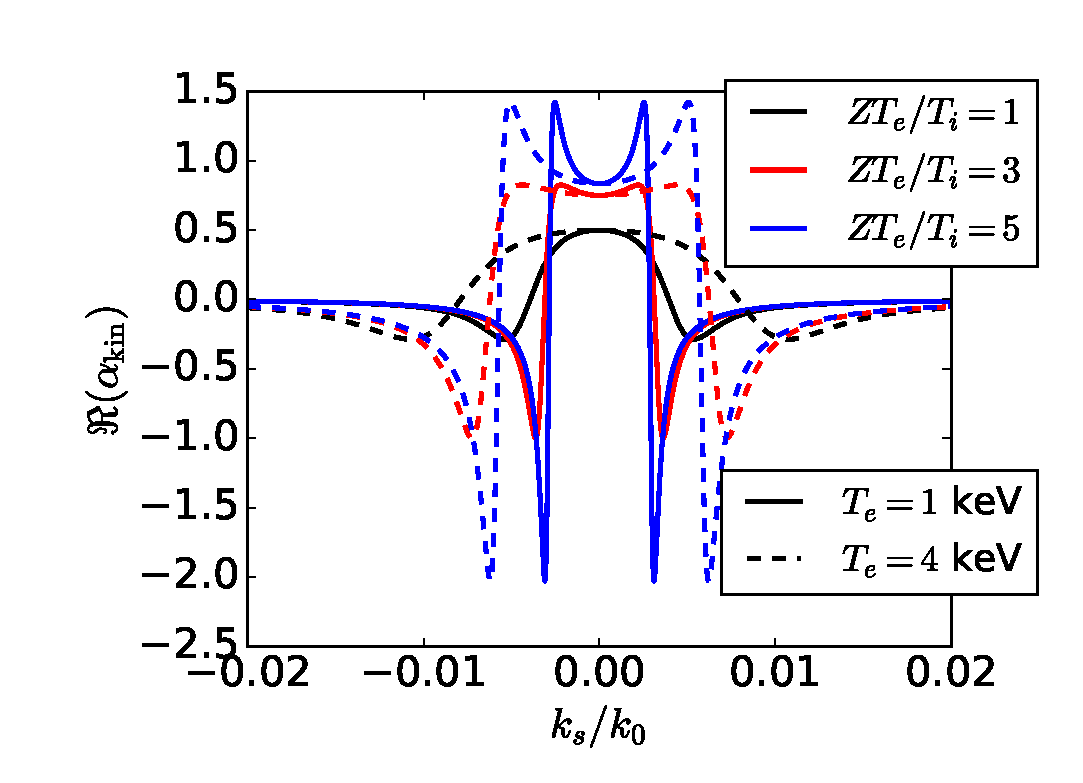
\includegraphics[width=0.49\textwidth]{akin.eps}\\
(b) $D=2$, $T_e=1$ keV, $ZT_e/T_i=3$\\
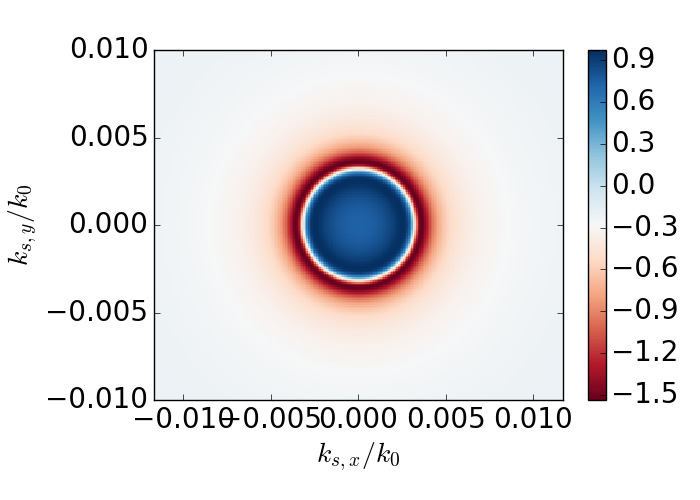
\includegraphics[width=0.49\textwidth]{akinD2.png}
\end{tabular}
\caption{ \label{fig:akin}  
 $\Re \left( \alpha_\mathrm{kin}   \right)$ for $D=1$ (a) and $D=2$ (b) as function of $k_s/k_0$ for a H$^{+}$ plasma with $n_0=0.1n_c$, $T_e =1$ keV for various $ZT_e/T_i$. 
 }
\end{figure}
In a 2D system ($D=1$), Fig. \ref{fig:akin} illustrates, for $D=1$ and for  a H$^{+}$ plasma with $n_0=0.1n_c$ and  $T_e =1$ keV, that $\Re \left( \alpha_\mathrm{kin}   \right)$ is an even function  of $k_s/k_0$ of width that enlarges as  $T_e$ increases. Moreover, its value vanishes for $\vert k_s/k_0 \vert  \gtrsim 2 \cdot 10^{-2}$, showing that the plasma is sensitive  to the very large wavelength perturbations ($\lambda_s/\lambda_0=k_0/k_s\gtrsim 314 $ or $k_s/k_0\lesssim 0.02$).
\textcolor{red}{Asymmetry 2D 3D.}
As there is, in  the system of interest here no privileged scattering direction, both stokes and antistokes plasma response modes have to be taken into account [see Eq. \eqref{eq:sa}]. Hence,  the resulting diffraction pattern  in the case of FSBS is  a stationary  wave, unlike CBET where it is fully propagating.

\subsection{Derivation of an effective growth rate relevant for an  RPP beam}
 \begin{widetext}
We may now combine the kinetic plasma response  with the paraxial model of  the laser propagation. 
However, it  is easier at this stage to introduce $\Bar{E}$ with  $E=\Bar{E}\exp(-i \mathbf{k}^2x /2k_0)$ so that Eq. \eqref{eq:parax} becomes
\begin{equation}
    \partial_x \Bar{E}  =\frac{-ik_0n_0}{2n_c} e^{\frac{i\mathbf{k}^2x }{2k_0}}\int \frac{d^Dk_s}{(2\pi)^D} \frac{\delta n(\mathbf{k}_s)}{n} \Bar{E}^\star(\mathbf{k}-\mathbf{k}_s) e^{ \frac{i(\mathbf{k}-\mathbf{k}_s)^2x}{2k_0}}\, ,  \label{eq:paraxbar}
\end{equation}
 plugged in Eq. \eqref{eq:drakef}, we obtain
\begin{align}
    \partial_x \Bar{E}  =\frac{ik_0n_0}{4n_c} \frac{e^{\frac{i\mathbf{k}^2 x}{2k_0}}}{  v_g n_c T_e}
    %\times \nonumber \\
    \int \frac{d^Dk_s}{(2\pi)^D}  e^{ \frac{i(\mathbf{k}-\mathbf{k}_s)^2x}{2k_0}} \Bar{E}^\star(\mathbf{k}-\mathbf{k}_s) 
   I_d(\mathbf{k}_s) \alpha_\mathrm{r}   (\mathbf{k}_s) 
   -\frac{ik_0n_0}{2n_c} e^{\frac{i\mathbf{k}^2x }{2k_0}}\int \frac{d^Dk_s}{(2\pi)^D} \mathcal{N}(\mathbf{k}_s) \Bar{E}^\star(\mathbf{k}-\mathbf{k}_s) e^{ \frac{i(\mathbf{k}-\mathbf{k}_s)^2x}{2k_0}}\, ,  \label{eq:paraxbar}
\end{align}
where we introduced $\alpha_\mathrm{r}=\Re(\alpha_\mathrm{kin} )$ and $\beta_r$. 

%\onecolumngrid
 When retaining only the first order terms (as $E_d$, $I_d$ and $\mathcal{N}$; $I_p$ and $E_p$ are considered of order zero), we obtain 
 \begin{align}
   e^{-i\omega_s t}\partial_x \Bar{E}_d  =&\frac{ik_0n_0}{4n_c} \frac{e^{\frac{i\mathbf{k}^2 x}{2k_0}}}{  v_g n_c T_e} \times 
   \int \frac{d^Dk_s}{(2\pi)^D} 
   e^{ \frac{i(\mathbf{k}-\mathbf{k}_s)^2x}{2k_0}}
   I_d(\mathbf{k}_s) \alpha_\mathrm{r}   (\mathbf{k}_s) \Bar{E}_p^\star(\mathbf{k}-\mathbf{k}_s) \nonumber\\
    &-\frac{ik_0n_0}{2n_c} e^{\frac{i\mathbf{k}^2x }{2k_0}}\int \frac{d^Dk_s}{(2\pi)^D} \mathcal{N}(\mathbf{k}_s) \Bar{E}_p^\star(\mathbf{k}-\mathbf{k}_s) e^{ \frac{i(\mathbf{k}-\mathbf{k}_s)^2x}{2k_0}}
   \, .  \label{eq:paraxbar}
\end{align}

In order to shade light on the dependence of the diffusion growth on the laser energy scattering direction, one needs to combine the above relation with the definition of $I_d(\mathbf{k})$ of  Eq. \eqref{eq:id}, which can be recast as,
\begin{align}
I_p(\mathbf{k}_d) &\simeq  \frac{c\epsilon_0}{2}  \int d^Dk \Bar{E}_p(\mathbf{k})
e^{\frac{ -i\mathbf{k}^2x}{2k_0}-i\omega_s t}
\Bar{E}_p^\star(\mathbf{k}_d-\mathbf{k})
e^{\frac{ i(\mathbf{k}_d-\mathbf{k})^2x}{2k_0}} 
  \, , \label{eq:ipb} \\
I_d(\mathbf{k}_d) &\simeq  \Re\left[  c\epsilon_0  \int d^Dk \Bar{E}_d(\mathbf{k})
e^{\frac{ -i\mathbf{k}^2x}{2k_0}-i\omega_s t}
\Bar{E}_p^\star(\mathbf{k}_d-\mathbf{k})
e^{\frac{ i(\mathbf{k}_d-\mathbf{k})^2x}{2k_0}} 
\right]  \, , \label{eq:idb} 
\end{align}
hence
\begin{align}
\partial_xI_d(\mathbf{k}_d)=  &  c\epsilon_0  \Re\left( \int d^Dk e^{-i\omega_st+ \frac{i( \mathbf{k}_d^2-2\mathbf{k}_d\cdot \mathbf{k} )x}{2k_0}} \Bar{E}_p^\star(\mathbf{k}_d-\mathbf{k} )
\left[\partial_x \Bar{E}_d (\mathbf{k}  ) 
+i\frac{  \mathbf{k}_d^2-2\mathbf{k}_d\cdot \mathbf{k}}{2k_0} \Bar{E}_d(\mathbf{k})
\right]  \right)\, , \label{eq:idbdz}
\end{align}
where the variations along $x$ of $\Bar{E}_p$ were neglected. 
The  use of Eq. \eqref{eq:paraxbar} yields, 
\begin{align}
\partial_xI_d(\mathbf{k}_d)\simeq &\Re\Big( \frac{ik_0n_0}{4n_c} \frac{c\epsilon_0 }{  v_g n_c T_e}   \int d^Dk \int \frac{d^Dk_s}{(2\pi)^D} \Bar{E}_p^\star(\mathbf{k}_d-\mathbf{k})
e^{\frac{i(\mathbf{k}-\mathbf{k}_s)^2x}{2k_0} }
e^{\frac{i(\mathbf{k}_d-\mathbf{k})^2x}{2k_0} }
I_d(\mathbf{k}_s) \alpha_\mathrm{r}(\mathbf{k}_s) 
\Bar{E}_p^\star(\mathbf{k}-\mathbf{k}_s) 
 \Big) \nonumber\\
+& c\epsilon_0  \Re\left(-\frac{ik_0n_0}{2n_c}  \int d^Dk\int \frac{d^Dk_s}{(2\pi)^D} e^{\frac{i( \mathbf{k}_d-\mathbf{k} )^2x}{2k_0}} \Bar{E}_p^\star(\mathbf{k}_d-\mathbf{k} )
%
%e^{\frac{i\mathbf{k}^2x }{2k_0}} 
\mathcal{N}(\mathbf{k}_s) \Bar{E}_p^\star(\mathbf{k}-\mathbf{k}_s) e^{ \frac{i(\mathbf{k}-\mathbf{k}_s)^2x}{2k_0}}
%
%\partial_x \Bar{E}_d (\mathbf{k}  ) 
%
  \right) \nonumber\\
& +c\epsilon_0  \Re\left( \int d^Dk e^{-i\omega_s t+\frac{ i( \mathbf{k}_d^2-2\mathbf{k}_d\cdot \mathbf{k} )x}{2k_0}} 
i\frac{  \mathbf{k}_d^2-2\mathbf{k}_d\cdot \mathbf{k}}{2k_0} \Bar{E}_d(\mathbf{k})\Bar{E}_p^\star(\mathbf{k}_d-\mathbf{k} )
  \right)
\, . \label{eq:g1}
\end{align}
Plugging Eqs. \eqref{eq:ipb}-\eqref{eq:idb} and retaining only the symmetric terms in the quadratures, 
\begin{align}
\partial_xI_d(\mathbf{k}_d)\simeq \Re\Big( \frac{ik_0n_0}{4n_c} \frac{1 }{  v_g n_c T_e}    \int \frac{d^Dk_s}{(2\pi)^D} I_d(\mathbf{k}_s) \alpha_\mathrm{r}(\mathbf{k}_s)
\Tilde{I}_p(\mathbf{k}_d-\mathbf{k}_s)
+\frac{i\mathbf{k}_d^2}{2k_0} I_d  - S(\mathbf{k}_d)\Big)
\, , \label{eq:g2}
\end{align}
where we defined 
\begin{align}
\Tilde{I}_p(\mathbf{k}_d-\mathbf{k}_s)  &=  c\epsilon_0  \int d^Dk \Bar{E}_p^\star (\mathbf{k}_d-\mathbf{k})
e^{\frac{ i (\mathbf{k}_d-\mathbf{k})^2x}{2k_0}-i\omega_s t}
\Bar{E}_p^\star(\mathbf{k}-\mathbf{k}_s)
e^{\frac{ i(\mathbf{k}-\mathbf{k}_s)^2x}{2k_0}}   \, , \label{eq:ipt} 
\end{align}
 and 
 \begin{align}
S(\mathbf{k}_d) =   \frac{ik_0n_0}{n_c} \int \frac{d^Dk_s}{(2\pi)^D}  
\mathcal{N}(\mathbf{k}_s)\Tilde{I}_p(\mathbf{k}_d-\mathbf{k}_s)
\, . \label{eq:s} 
\end{align}
It is important to note that $\Tilde{I}_p$ differs from $I_p$, and, in order to progress, an assumption on the nature of the pump wave has to be made. 

 \subsection{Energy growth of the Forward Brillouin scattering for an RPP beam }
%For symmetric scattering, the last term  of the above equation may be neglected and, defining $\Bar{I}_d$ through $I_d = \Re[\Bar{I}_d\exp(i\mathbf{k}_d^2x/2k_0)]$, one obtains
% \begin{align}
%\partial_x\Bar{I}_d(\mathbf{k}_d)\simeq  \frac{ik_0n_0}{2n_c} \frac{e^{\frac{-i\mathbf{k}_d^2x}{2k_0}} }{  v_g n_c T_e}   
%  \int \frac{d^Dk_s}{(2\pi)^D} \Bar{I}_d(\mathbf{k}_s) \alpha_\mathrm{r}(\mathbf{k}_s) 
%I_p(\mathbf{k}_d-\mathbf{k}_s)
%e^{\frac{i\mathbf{k}_s^2x}{2k_0}} 
%\, . \label{eq:g3}
%\end{align}
%It is essential to notice that, if diffraction had been neglected, thus removing the exponential terms of the above equations, the real part of $\partial_x \Bar{I}_d$ would be vanishing, implying no growth of the scattered wave. Hence, accounting for diffraction, \emph{i.e.} the curvature of the off focus wave front,  is crucial for modeling the Forward stimulated Brillouin scattering.
 Using the  RPP  beam model of Refs. \cite[]{POF_Schmitt_88,POF_Rose_93},
 \begin{align}
 \Bar{E}_p(\mathbf{k}) = \frac{E_0}{N} \sum_{n,\vert k_{\perp,y/z}(n)\vert<k_m } e^{i\Phi_{\mathbf{k}_\perp}}\delta(\mathbf{k}  - \mathbf{k}_\perp(n))\, , \label{eq:erpp}
 \end{align}
 where  $N$ is the number of diffracting elements, 
 $\delta(x)$ the Dirac function and the phases $\Phi_{k_y}$,  independent random variables taking the values $0$ or $\pi$ with equal probability.
 For simplicity, we will assume a square phase plate that verifies $k_{\perp,y/z}(n) = n2k_m/N$ with $n$ an integer that verifies $n\in \llbracket - N/2 ,N/2 \rrbracket$. 
 Under these conditions, and for $\langle x\rangle$ representing the statistical average of $x$,  we note   that $\langle\exp(i\Phi_{k_1}+i\Phi_{k_1})\rangle=\delta(k_1-k_2) $ so that  the statistical average  of Eq. \eqref{eq:ip} verifies
   \begin{align}
   \langle I_p(\mathbf{k})\rangle &= I_0 \sigma ^D \mathcal{H}^{(D)}(\mathbf{k})  &\,  \mathrm{with} \, ,\\ 
   \mathcal{H}^{(1)}(\mathbf{k}) &= H(2k_m - \vert k_y \vert ) &\,  \mathrm{in}\, \mathrm{2D} \, ,\\ 
    \mathcal{H}^{(2)}(\mathbf{k}) &=   H(2k_m - \vert k_y \vert ) H(2k_m - \vert k_z \vert ) &\,  \mathrm{in}\, \mathrm{3D} \, .
   \end{align}
We introduce,  $H$ the step function, $k_m=k_0/2f$ with $f$ the effective speckle focal number,  and $\sigma$ the transverse size of the pump wave, \emph{i.e.}, $I_0\sigma^D$ is its initial power.
As, for $\Tilde{I}_p$, its statistical average for an RPP beam reads, 
\begin{align}
\langle \Tilde{I}_p(\mathbf{k}_d-\mathbf{k}_s)\rangle   &=  c\epsilon_0\frac{E_0^2}{N^2}  \int d^Dk 
e^{\frac{ i (\mathbf{k}_d-\mathbf{k})^2x}{2k_0}-i\omega_s t}
e^{\frac{ i(\mathbf{k}-\mathbf{k}_s)^2x}{2k_0}}  
\sum_{\vert k_{1,y/z}\vert,\vert k_{2,y/z}\vert  <k_m}
\langle e^{i\Phi_{\mathbf{k}_1}+i\Phi_{\mathbf{k}_2}}\rangle
\delta(\mathbf{k}_d-\mathbf{k} -\mathbf{k}_2 ) 
\delta(\mathbf{k}-\mathbf{k}_s -\mathbf{k}_1) 
\, . \label{eq:ipt2} 
\end{align}
When  $\mathbf{k}_1=\mathbf{k}_2$, the Dirac functions can be recast into 
\begin{align}
\delta(\mathbf{k}_d-\mathbf{k} -\mathbf{k}_2 ) 
\delta(\mathbf{k}-\mathbf{k}_s -\mathbf{k}_1)= \mathcal{H}^{(D)}(2\mathbf{k}-2\mathbf{k}_s  )  \delta (\mathbf{k}_d+\mathbf{k}_s -2\mathbf{k} ) \, ,
\end{align}
and thus yields
\begin{align}
\langle \Tilde{I}_p(\mathbf{k}_d-\mathbf{k}_s)\rangle   &=  I_0\sigma^D
e^{\frac{ i(\mathbf{k}_d-\mathbf{k}_s)^2x}{4k_0}}  
\mathcal{H}^{(D)}\left( \mathbf{k}_d-\mathbf{k}_s  \right)
\, . \label{eq:iptf} 
\end{align}
Hereafter, the $\langle  \cdot \rangle$-notation will  me removed for sake of simplicity. 
Equations \eqref{eq:g2} and \eqref{eq:iptf} may now be combined,  
  \begin{align}
\partial_xI_d(\mathbf{k}_d)&\simeq  \Re\left( \frac{ik_0n_0}{2n_c} \frac{ I_0\sigma^D }{  v_g n_c T_e}   
 \int \frac{d^Dk_s}{(2\pi)^D}   \mathcal{H}^{(D)}(\mathbf{k}_d-\mathbf{k}_s) I_d(\mathbf{k}_s) \alpha_\mathrm{r}(\mathbf{k}_s) e^{\frac{ i(\mathbf{k}_d-\mathbf{k}_s)^2x}{4k_0}}  -S(\mathbf{k}_d) \right)
\, . \label{eq:g4}\\
S(\mathbf{k}_d) &=   \frac{ik_0n_0}{n_c} I_0\sigma^D\int \frac{d^Dk_s}{(2\pi)^D}  \mathcal{H}^{(D)}\left( \mathbf{k}_d-\mathbf{k}_s  \right)
\mathcal{N}(\mathbf{k}_s) e^{\frac{ i(\mathbf{k}_d-\mathbf{k}_s)^2x}{4k_0}}  
\end{align}

Since $2k_m$ is much larger than the width of $\alpha_r(k_s)$, we may use $\int_{k_d-2k_m}^{k_d+2k_m} X \simeq \mathcal{H}^{(1)}(k_d) \int_{-\infty}^{+\infty}X$. For simplicity, the same assumption will be applied to the seed term $S$, and, introducing $\delta n/n_c=n_0I_0/{n_c^2 T_ev_g}$ we obtain, 
 \begin{align}
\partial_xI_d(\mathbf{k}_d)&\simeq  \frac{-k_0}{2} \frac{ \delta n}{n_c}   \sigma^D
 \mathcal{H}^{(D)}(\mathbf{k}_d)
 \int \frac{d^Dk_s}{(2\pi)^D}    [I_d(\mathbf{k}_s) \alpha_\mathrm{r}(\mathbf{k}_s) - I_s(\mathbf{k}_s)] \sin\left[{\frac{ (\mathbf{k}_d-\mathbf{k}_s)^2x}{4k_0}}  \right]
\, ,  \label{eq:g5}\\
I_s(\mathbf{k}_s) &=-2n_c T_ev_g   
\mathcal{N}(\mathbf{k}_s)
\end{align}
%In order to reach analytical progress, we will assume that $I_d$ is  smoother and larger  than $\alpha_\mathrm{r}(\mathbf{k}_s) 
%\sin[(\mathbf{k}_d^2-\mathbf{k}_s^2)x / 2k_0]$, hence
%\begin{align}\partial_xI_d(\mathbf{k}_d)\simeq  \frac{-k_0}{2} \frac{ \delta n}{n_c}   \sigma^D\mathcal{H}^{(D)}(\mathbf{k}_d) I_d(0) \int \frac{d^Dk_s}{(2\pi)^D}    \alpha_\mathrm{r}(\mathbf{k}_s) \sin\left[{\frac{ (\mathbf{k}_d-\mathbf{k}_s)^2x}{4k_0}}  \right]\, . %\label{eq:dxidkd}
%\end{align}
 
 \begin{figure*}[!]
\begin{tabular}{cc}
(a) $D=1$ &(b) $D=2$ \\
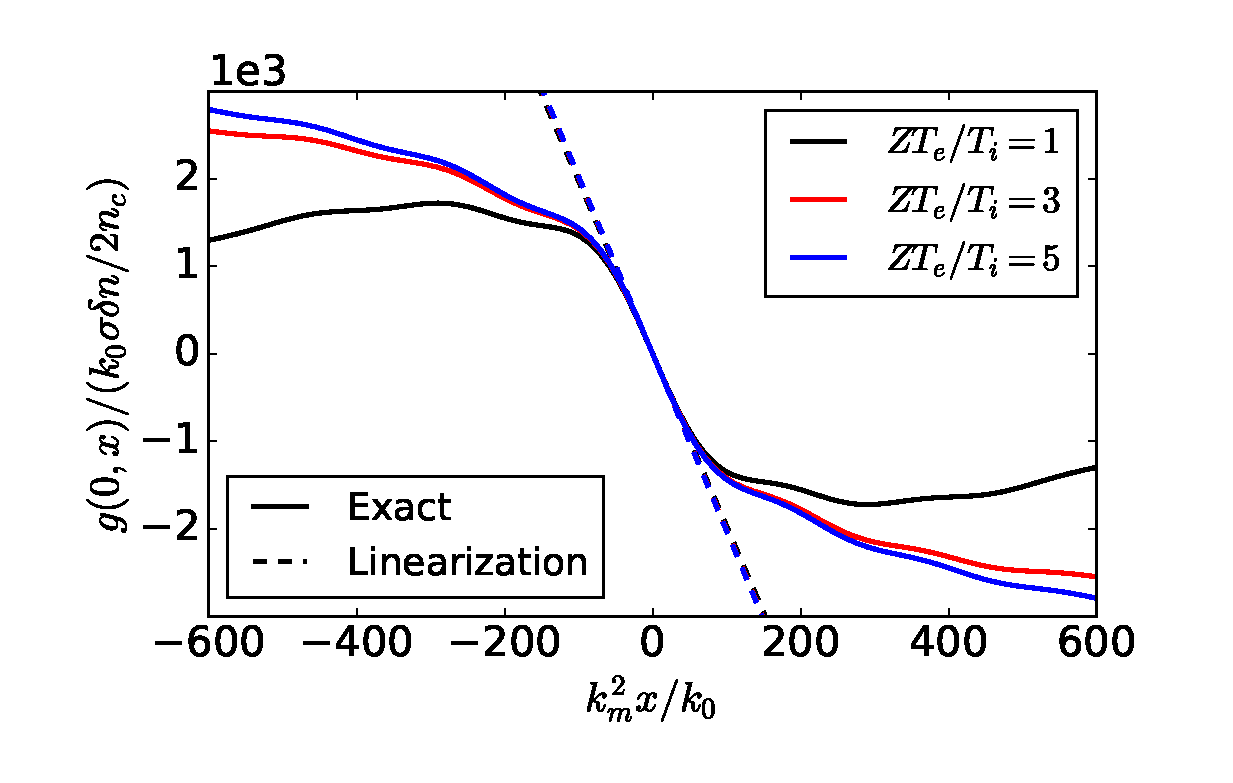
\includegraphics[width=0.49\textwidth]{int_akin_sin.eps}
 &
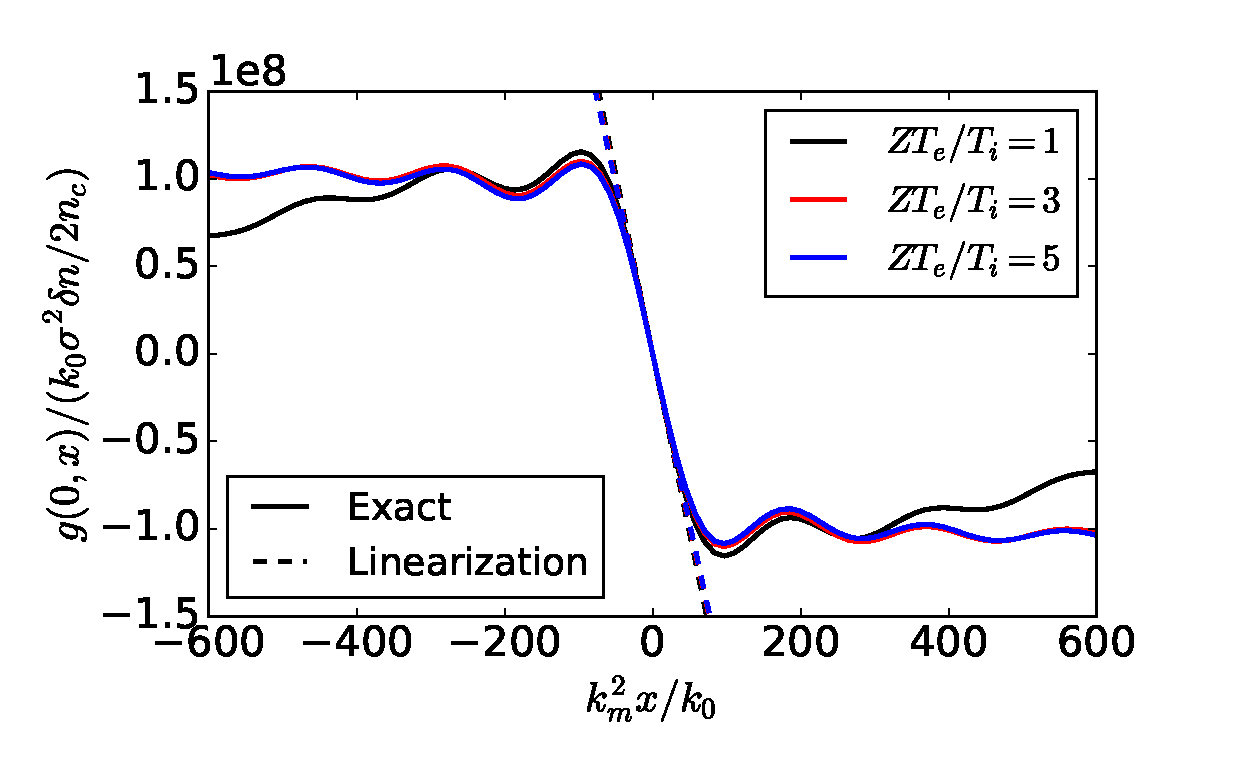
\includegraphics[width=0.49\textwidth]{int_akin_sin_D2.eps}
\end{tabular}
\caption{ \label{fig:intakinsin}
Numerical calculation of $g_0(x)$ by Eq. \eqref{eq:gain0} for $\sigma = 200 \,\mu m$ and  for various values of $ZT_e/T_i$ in the case $D=1$ (a) and $D=2$ (b). 
 }
\end{figure*}
%\begin{align}
%g(\mathbf{k}_d,x) = \frac{\partial_x I_d(\mathbf{k}_d)}{I_d(0)} %\nonumber \\
%=  \frac{-k_0}{2} \frac{ \delta n}{n_c}   \sigma^D
% \mathcal{H}^{(D)}(\mathbf{k}_d)
% \int \frac{d^Dk_s}{(2\pi)^D}    \alpha_\mathrm{r}(\mathbf{k}_s) \sin\left[{\frac{ (\mathbf{k}_d-\mathbf{k}_s)^2x}{4k_0}}  \right]\, . \label{eq:gainkd}
%\end{align}

%Making use of 
%\begin{align}
    %\int_{-2k_m}^{+2k_m}dk\sin\left[{\frac{ (k-k_s)^2x}{4k_0}}  \right]=\sqrt{\frac{2\pi k_0}{x}}\left[ \mathrm{S}\left(\sqrt{\frac{x}{2\pi k_0}} (2k_m- k_s)\right)-\mathrm{S}\left(\sqrt{\frac{x}{2\pi k_0}} (-2k_m -k_s)\right)\right]
%\end{align}
 \end{widetext}
Deriving the exact and general solution of the above equation is out of the scope of this manuscript, however, interesting results may emerge from tractable limits. 

 \subsection{Angular dependence of the  Forward Brillouin scattering}
As a the plateau width of $\alpha_r$ is much smaller than $2k_m$,\textcolor{red}{(Demonstration generale)}  we may assume, in the quadrature of Eq. \eqref{eq:g5},   $ \vert\mathbf{k}_s \vert/\vert\mathbf{k}_d\vert \le\Delta k/ \vert\mathbf{k}_d\vert \ll 1$ so that to leading order,
\begin{align}
\partial_xI_d(\mathbf{k}_d,x)&\simeq  \frac{-k_0}{2} \frac{ \delta n}{n_c}   \sigma^D 
 \mathcal{H}^{(D)}\sin\left({\frac{ \mathbf{k}_d^2x}{4k_0}}  \right)
B(x)
\, , \label{eq:dxidtd}
\end{align}
where $B(x)$ is,
\begin{align}
B(x)&=
 \int \frac{d^Dk_s}{(2\pi)^D}    I_d(\mathbf{k}_s) \alpha_\mathrm{r}(\mathbf{k}_s) 
\, . \label{eq:b}
\end{align}
With $g_0(x)$ following
\begin{align}
g_0(x)&= -\Gamma_0 \int \frac{d^Dk_s}{(2\pi)^D}  \alpha_\mathrm{r}(\mathbf{k}_s) 
\sin\left(\frac{ \mathbf{k}_s^2x}{4k_0}  \right)\,  \nonumber\\
\Gamma_0&=\frac{k_0}{2}  \frac{\delta n}{n_c}
  \sigma^D \, ,
\label{eq:gain0}
\end{align}
one can easily show that $B(x)$ fulfills 
\begin{align}
d_xB = g_0(x) B(x)\, ,
\label{eq:db}
\end{align} 
and thus, for a left boundary located at $x=x_0$,
\begin{align}
B(x) = B_0\exp\left(\int_{x_0}^x g_0 \right)\, ,
\label{eq:bf}
\end{align} 
where $B_0$ is an integration constant independent of the wavevector.

Combining Eqs.  \eqref{eq:dxidtd} and \eqref{eq:bf} yields 
\begin{align}
\partial_xI_d(\mathbf{k}_d,x)&\simeq -B_0\Gamma_0
 \mathcal{H}^{(D)}\sin\left({\frac{ \mathbf{k}_d^2x}{4k_0}}  \right)
\exp\left(\int_{x_0}^x g_0 \right)
\, . \label{eq:dxidtdf}
\end{align}

Figures \ref{fig:intakinsin}(a,b) illustrate, as a function of $k_m^2 x /k_0$, the evolution of $g_0(x)$
normalized to $\Gamma_0=k_0\delta n / 2n_c$. Note that, for $\lambda_0=2\pi/k_0=0.35\,\rm\mu m$ and $f=6.5$,  $k_m^2 x /k_0=200$ corresponds to $x\simeq 2\,\rm mm$. 
The value of $g_0$ is negative before focus (\emph{i.e.} $x=0$) and positive afterward, with  a linear behavior of the $g(0,x)$ for  $\vert k_m^2 x /k_0 \vert < 200$  independent of $ZT_e/T_i$. In both cases $D=1$ and $2$, the slope of $g_0(x)$  in the vicinity of $x=0$   decreases significantly when   $\vert k_m^2 \vert x\vert /k_0 \vert \gtrsim 100$, this occurs when the $\sin(k^2x/4k_0)$ in the quadrature of Eq. \eqref{eq:gain0} varies faster than the plateau width of $\alpha_r$, $\vert k_s/k_0\vert \lesssim 5\cdot 10^{-3}\equiv \Delta k /2$ in Figs. \ref{fig:akin}(a,b), \emph{i.e.} for $\vert x\vert \gtrsim 2k_0/\Delta k^2$ which gives $\vert k_m^2x/k_0 \vert  \gtrsim 120  $ in reasonable  agreement with Figs. \ref{fig:intakinsin}(a,b).
For both dimensions and$\vert k_m^2 x /k_0 \vert \gtrsim 400$, the absolute value of $g_0(x)$ vanishes faster as $ZT_e/T_i$ decreases. 

Interestingly, when $ZT_e/T_i=1$ and $T_e=4$ kev, $g_0$ become positive for $k_m^2x/k_0<-400$, \emph{i.e.} well before focus (at $x=0$). In this region,  the $\sin(k^2x/4k_0)$ in the quadrature of Eq. \eqref{eq:gain0} is minimized   where $\alpha_r$ reaches its minimum [see Fig. \ref{fig:akin}(a), $\vert k_s/k_0\vert \simeq 0.01$ for $ZT_e/T_i=1$ and $T_e=4$ kev in dashed black line]. Indeed, plugging  $\vert k_s/k_0\vert \simeq 0.01$ into $3\pi/2>k^2x/4k_0>\pi/2$ results in a positive value of $g_0$  when $1100\gtrsim \vert x\vert\gtrsim 370$, in agreement with Figures \ref{fig:intakinsin}(a) (dashed black line).
Note that if the Forward stimulated Brillouin  scattering were to grow   and affect the pump propagation more than four millimeters before focus, a large impact on the pump propagation and its energy deposition is to be expected. 

Let's momentarily consider, for illustration purposes,  the  case of a RPP beam of width $\sigma =200\,\rm\mu m$, $I_0=3\cdot 10^{14} \,\rm W.cm^{-2}$, $2\pi/k_0 = 0.35\,\rm\mu m$ and $f = 6.5$ propagating in a H$^{+}$ plasma with $n_e/n_c=0.1$, , $T_e=1$ kev and $T_i=300$ eV. In these conditions, $\delta n/n_c \simeq 7\cdot 10^{-4}$ and  for $D=1$ [see Fig. \ref{fig:intakinsin}(a)], one have $g_0(x)/\Gamma_0 \gtrsim 3\cdot 10^3$ before focus (for $200< k_m^2 x/k_0 < 600$) so that, for  a propagation of $\Delta x = 2\,\rm mm$ (\emph{i.e.} $k_m^2 \Delta x/k_0 = 200$), the net gain is $g_0(x)\Delta x\sim 7 $. When $D=2$ [see Fig. \ref{fig:intakinsin}(b)], one obtains $g_0(x)\Delta x\sim 350 $, thus yielding substantial growth for both dimensions.

We therefore know that the Forward Brillouin may grow significantly in the plasmas  of interest here and, in order to shade light on the scattered  direction of the pump wave, we will now address the spectral behavior of Eq. \eqref{eq:dxidtdf}.

\section{Approximated and analytical formulation of the effective gain}
\subsection{The role of seed acoustic fluctuations on the growth of FSBS}
Whether $g_0$ is positive or negative,  the scattered intensity can grow following Eq. \eqref{eq:dxidtdf} ($\partial_x I_d>0$) provided that the wavevectors verify $\vert k_{x/y}\vert \le 2k_m$ and $-\sin( \mathbf{k}^2x/4k_0 ) >0$.
However, when $g_0<0$ the exponential term in Eq. \eqref{eq:dxidtdf} rapidly damp the growth, keeping $I_d$ to negligible values or, physically, close to the self sustained noise level.   
Not capture by our model, the interplay between the thermal fluctuations (assuming they represent the   appropriate seed term) and the growth of the Forward Brillouin  requires to couple the above model with a source noise  \cite[]{Yoon_2007,Ruyer_Gremillet_2013} and is out of the scope of this manuscript. 
For this study we will settle for assuming that while $g_0<0$, $I_d$ is kept to a finite seed level. This ensues that that Eq. \eqref{eq:dxidtdf} will be hereafter applied replacing the left boundary location  $x=x_0$ by $x=x_c$ for which $g_0(x>x_c)\ge 0$. 

Regarding the unstable modes, the most growing wavevectors verifies  $\vert \mathbf{k}\vert =k_n$ with  $-\sin(k_n^2x/4k_0 ) =1$,
\begin{equation}\label{eq:kn}
    k_n^2(x) =\frac{4\pi k_0}{x} \left(2n- \frac{1}{2}   \right) \, .
\end{equation}
Here, $n$ is a signed  integer with  $n \cdot x /\vert x\vert\in  \llbracket 1 ,N_\mathrm{max} \rrbracket$ and  $ N_\mathrm{max}$ ensues from setting  $k_n=2k_m$ in Eq. \eqref{eq:kn},
\begin{equation}\label{eq:nmax}
    N_\mathrm{max} =\left\lfloor  \frac{k_m^2\vert x\vert }{2\pi k_0} +\frac{1}{4}   \right\rfloor \,  ,
\end{equation}
where $\lfloor u  \rfloor$ is the floor value of u. 
A total a $2N_\mathrm{max}$ that can be  amplified and are not regularly distributed in the the initial RPP spectral width $\vert k \vert< 2k_m$, most of them are located in $\vert k \vert >k_m\gg \Delta k$. 

\subsection{Forward Brillouin-unstable region after the focal plane}
We will here address the region $x>0$ for which Figs. \ref{fig:intakinsin}(a,b) presents $g_0>0$.
As $x$ grows starting from  $x=0$,  $\partial_x I_d$ starts to be positive  first for  $\vert k_{y/z} \vert= 2k_m$, if $2\pi>4k_m^2x/4k_0>\pi$, \emph{i.e.} when 
\begin{equation}\label{eq:xc}
x_c=x_1^- = \frac{\pi k_0 }{k_m^2}  <x < x_1^+ = \frac{2\pi k_0 }{k_m^2} \, .
\end{equation}
Moreover, the first most unstable mode, $k_1(x)$, enters in the  RPP spectral width $\vert k \vert< 2k_m$ when $k_1(x)=2k_m$ so that 
$x=3\pi k_0 /2k_m^2=(x_1^++x_1^-)/2$. As $x$ increases and become larger than $x_1^+$, more and more mode verifies $\vert k_{y/z} \vert= 2k_m$, and the number of unstable wavevectors increases linearly, following Eq. \eqref{eq:nmax}.

\subsubsection{Effective gain in the region $x_1^-<x<x_1^+$}
Making use of  $f=6.5$ and $2\pi/k_0=0.35\,\rm \mu m$ yields  $(x_1^-,x_1^+)= (30,60)\,\rm\mu m$  and  $f=6.5$ and $2\pi/k_0=1\,\rm \mu m$ results in $(x_1^-,x_1^+)= (84,168)\,\rm\mu m$. 
Hence, when $x_1^-<x<x_1^+$, the most unstable modes are located at $\vert k_{y/z}\vert= 2k_m$. In the vicinity of the focal plane, a Taylor development of  $g_0$ may be used assuming $\vert \Delta k^2x/4k_0\vert  \ll 1$,
\begin{align}
%g_0&\simeq -\Gamma_0 \left(\frac{A_2}{4k_0} x + \frac{A_6}{192k_0^3 }x^3 \right) \label{eq:g0td}\, ,\\ 
g_0&\simeq -\Gamma_0  \frac{A_2}{4k_0} x + O(x^3)  \label{eq:g0td}\, ,\\ 
A_n&=\int\frac{d^Dk_s}{(2\pi)^{D}}k_s^n\alpha_r \, . \label{eq:an}
\end{align}. 
Combined with Eq. \eqref{eq:dxidtdf}, for $x_1^-   <x < x_1^+$  we obtain,
\begin{align}
\partial_xI_d(2k_m)&\simeq -B_0\Gamma_0
\sin\left({\frac{ k_m^2x}{k_0}}  \right)
\exp\left(  - \frac{ \Gamma_0 A_2x^2}{8k_0}  \right)
\, , \label{eq:dxx0}
\end{align}
where $A_2<0$ for $ZT_e/T_i\ge 1$. 
\begin{figure}[!]
\begin{tabular}{cc}
(a) $\log_{10}[A(x_1^-,x_1^+)]$,  $D=1$\\
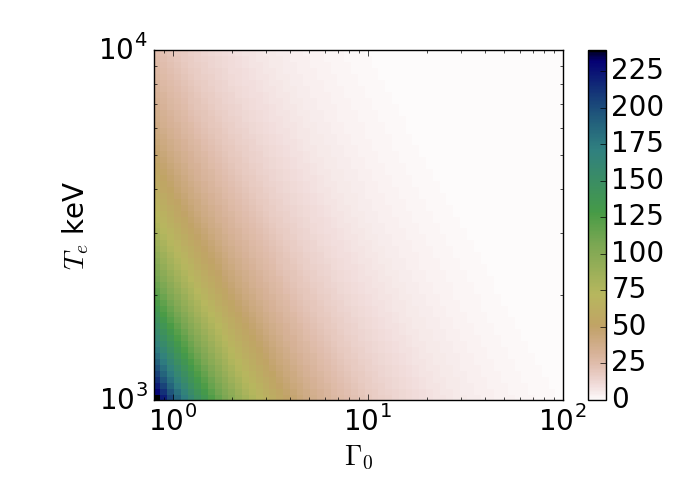
\includegraphics[width=0.49\textwidth]{Gx1_D2.png}\\
(b) $D=2$\\
%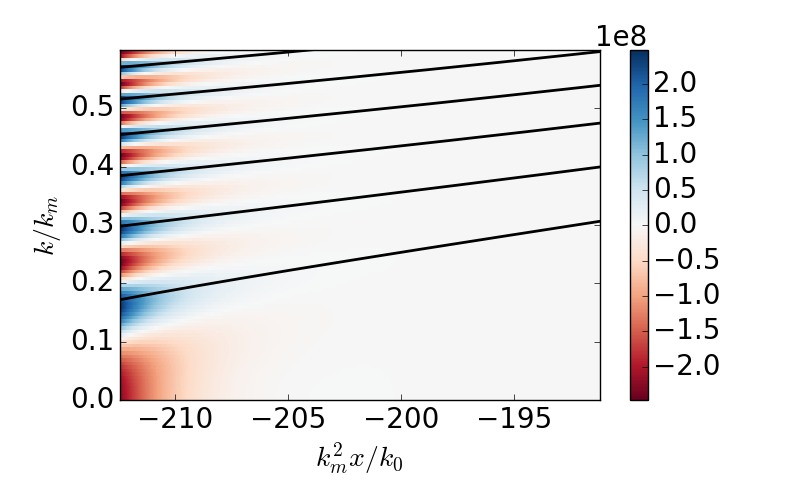
\includegraphics[width=0.49\textwidth]{gkx_2d_2mm_D2.png}\\
%(c)\\
%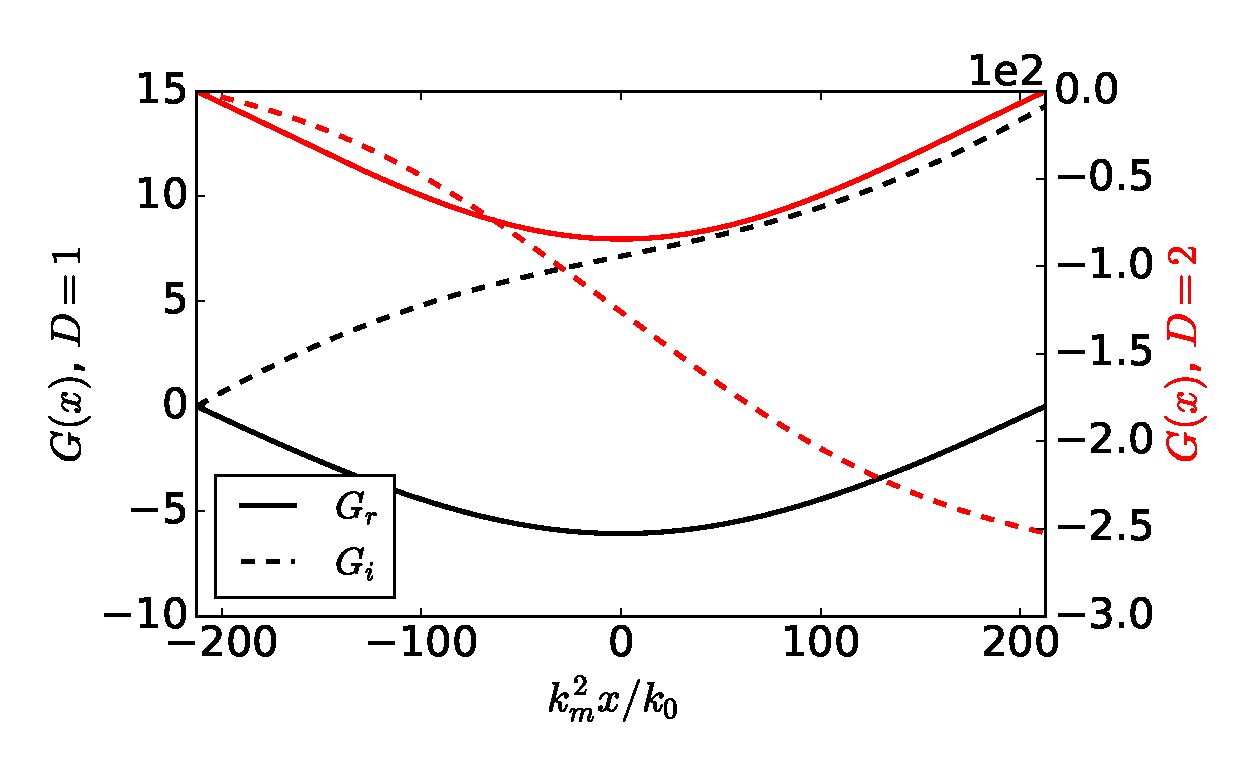
\includegraphics[width=0.49\textwidth]{G_2d_2mm.eps}
\end{tabular}
\caption{ \label{fig:gx1}
(a,b) 
 }
\end{figure}
The integration between $x_1^-$ and $x_1^+$ requires the introduction of a constant, $I_{d,0}=I_d(x=x_1^-)$, assumed to be independent of $k$ for simplicity and which can be related to $B_0$ [see Eq. \eqref{eq:b}] through $B_0=I_{d,0}A_0$, thus giving
\begin{widetext}
\begin{align}
 A(x_1^-,x_1^+)=\frac{I_d(2k_m,x_1^+)}{I_d(2k_m,x_1^-)} - 1& \simeq 
\frac{A_0\Gamma_0}{4} e^{-\frac{k_m^4 2\pi}{k_0  \Gamma_0A_2}}\sqrt{\frac{8\pi k_0}{-\Gamma_0A_2}}
\left[ 
\mathrm{erf}\left(\frac{
\frac{ k_m^2}{k_0} +i\frac{ \Gamma_0 A_2}{4k_0} z }{\sqrt{\frac{-\Gamma_0A_2}{2 k_0}}} \right)
+\mathrm{erf}\left(\frac{
\frac{ k_m^2}{k_0} -i\frac{ \Gamma_0 A_2}{4k_0} z }{\sqrt{\frac{-\Gamma_0A_2}{2 k_0}}} \right)
\right]_{z= \frac{\pi k_0 }{k_m^2} }^{z= \frac{2\pi k_0 }{k_m^2} }
\, . \label{eq:idx01}
\end{align}
\end{widetext}
Figure \ref{fig:gx1} illustrates $A(x_1^-,x_1^+)=I_d(2k_m,x_1^+) / I_d(2k_m,x_1^-) - 1$ in logarithmic scale for $ZT_e/Ti=3$. Note that the dependency of $A(x_1^-,x_1^+)$ on $ZT_e/Ti$ are found to be weak.
A  large effective gain of the scattered intensity  $\sim 100$ is evidenced for  $T_e<3$ keV and $\Gamma_0<2$ ($D=1$) although it might be overestimated due to  the  Taylor development of Eq. \eqref{eq:g0td}.

%Assuming $g_0$ varies slower than $-\sin( \mathbf{k}^2x/4k_0 ) >0$ in Eq. \eqref{eq:dxidtdf}, 
\textcolor{red}{!!!!!!}

%\begin{figure}[!]
%\begin{tabular}{cc}
%(a) $D=1$\\
%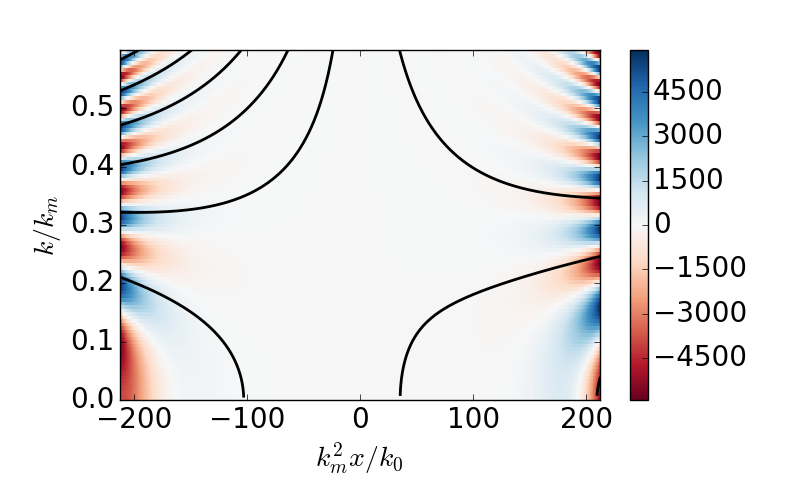
\includegraphics[width=0.49\textwidth]{gkx_2d_2mm.png}\\
%(b) $D=2$\\
%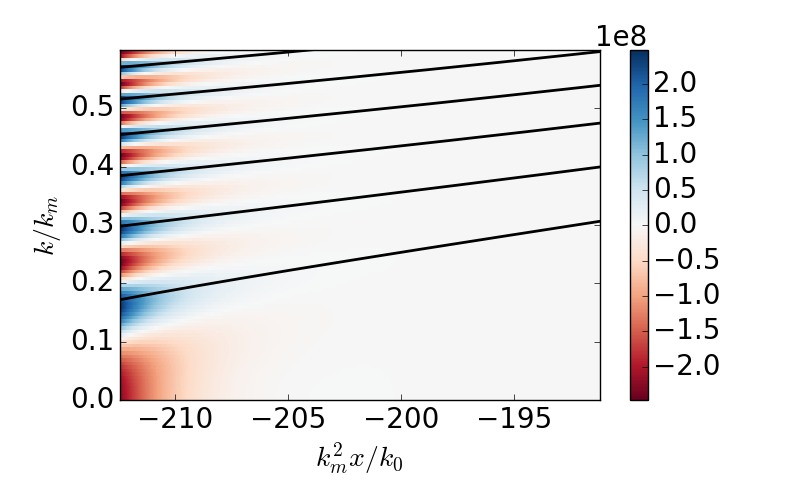
\includegraphics[width=0.49\textwidth]{gkx_2d_2mm_D2.png}\\
%(c)\\
%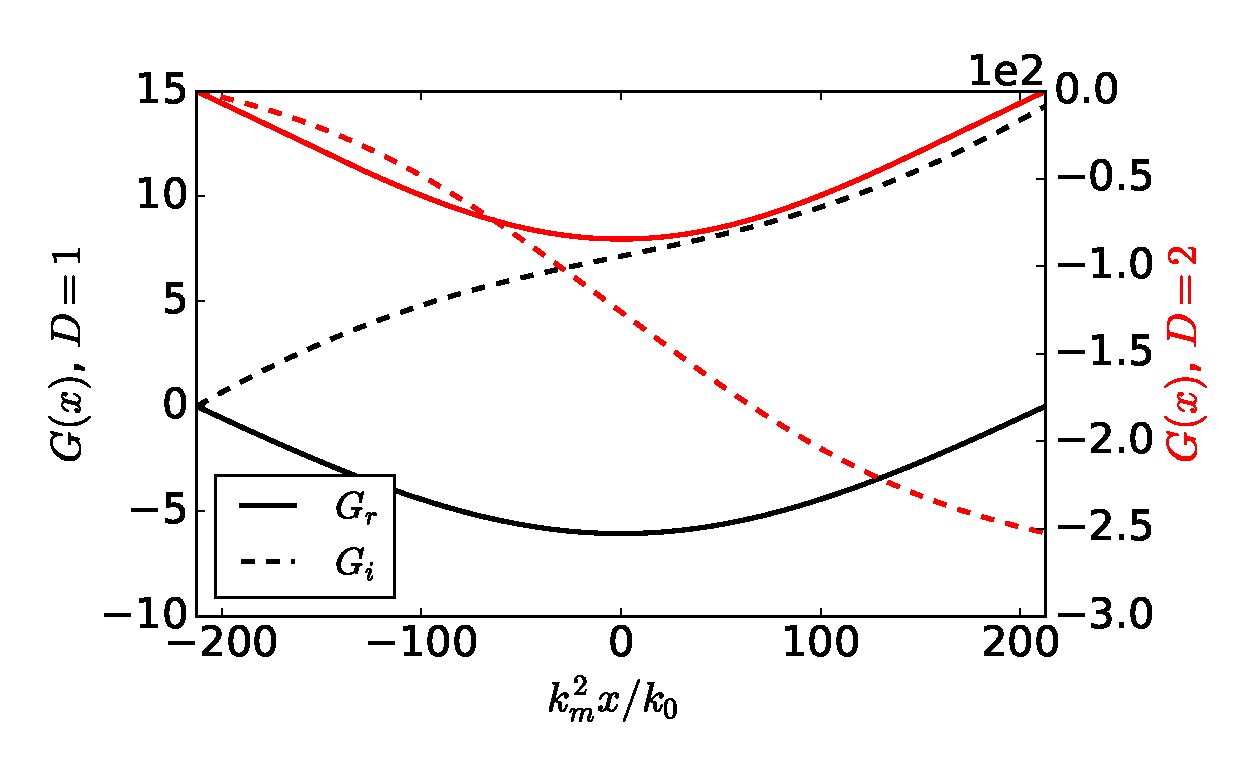
\includegraphics[width=0.49\textwidth]{G_2d_2mm.eps}
%\end{tabular}
%\caption{ \label{fig:gxk}
%(a,b) Numerical evaluation with $k_m^2x_0/k_0 = -212$ of $\partial_x I_d /I_{d,0}\Gamma_0$ following Eq. \eqref{eq:dxidkdf} for $(D,\Gamma_0)=(1,1.2)$ (a) and $(D,\Gamma_0)=(2,2.5\cdot 10^{-4} )$ (b) as a function of $k_m^2x/k_0$ and $k_d/k_m$.
%(c) $G(x)$ for $D=1$ (black, left axis) and $D=2$ (red, right axis).
%The wavevector that maximizes $\partial_x I_d$  from Eq. \eqref{eq:kn} are superimposed on (a) and (b) as black plain lines.
% }
%\end{figure}

%For $(D,\Gamma_0)=(1,1.2)$,   or $(D,\Gamma_0)=(2,2.5\cdot 10^{-4} )$ (which corresponds to $\delta n/n_c =7\cdot 10^{-4}$, $2\pi/k_0=0.35\,\rm\mu m$ and $\sigma=200\,\rm\mu m$) and $k_m^2x_0/k_0= -200$ (\emph{i.e.} $x_0=-2 \,\rm mm$ for $2\pi/k_0=0.35\,\rm\mu m$ and $f=6.5$),

%\begin{figure}[!]
%\begin{tabular}{c}
%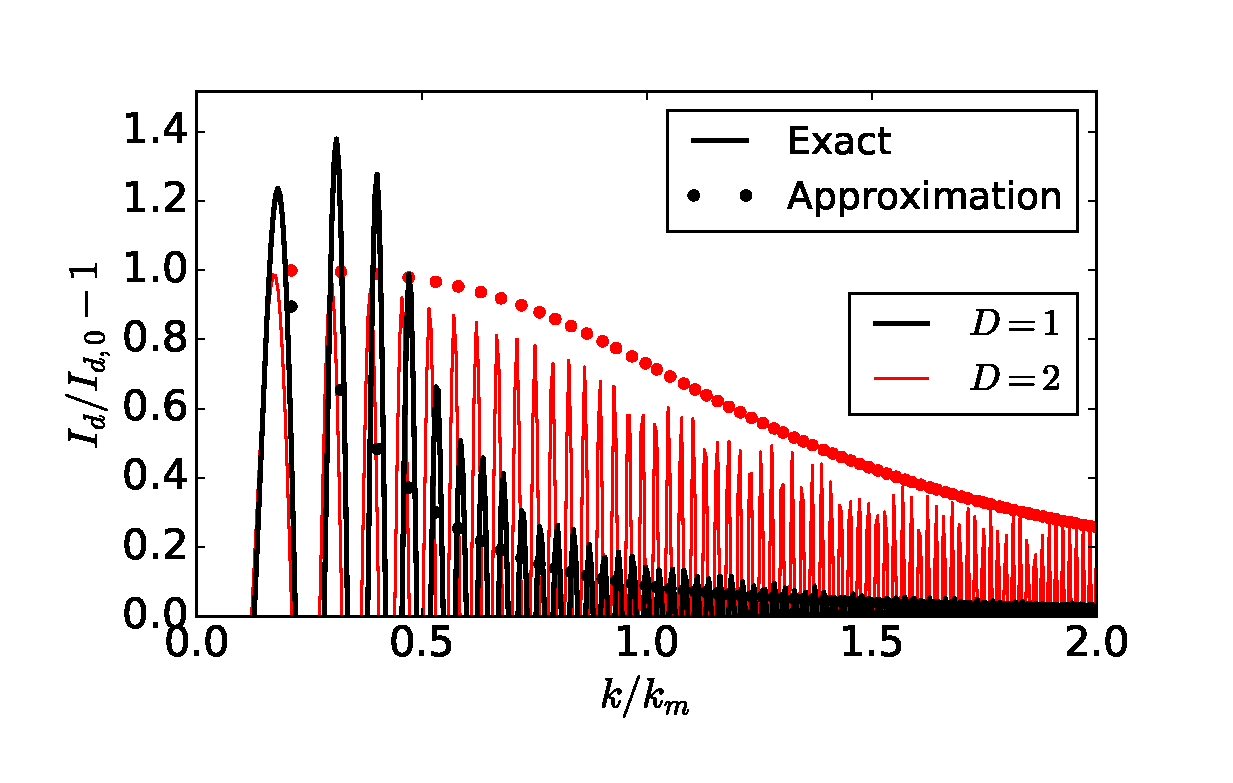
\includegraphics[width=0.49\textwidth]{Idk.eps}
%\end{tabular}
%\caption{ \label{fig:idk}
%Scattered intensity normalized to its initial value and the focal plane, $I_d(x=0)/I_{d,0}-1$ obtained through the numerical integration of Eq. \eqref{eq:dxidkd} in plain lines for 
%$\sigma =200\,\rm\mu m$, $I_0=3\cdot 10^{14} \,\rm W.cm^{-2}$, $2\pi/k_0 = 0.35\,\rm\mu m$,$f = 6.5$, $Z=A=1$, $n_e/n_c=0.1$, , $T_e=1$ kev and $T_i=300$ eV. The approximation of Eq. \eqref{eq:idtdamp} for $k=k_n$ are superimposed  as circles.
% }
%\end{figure}
%For the case of Fig. \ref{fig:gxk} and  at $x=x_0$, a total of $2(N_\mathrm{max}-N_\mathrm{min}+1) = 422$ growing modes are  found [only 6 of them verifies $0<k_n<0.6k_m$, see (a,b)]. As shown in  Fig. \ref{fig:idk} which illustrates $I_d(x=1, k)/I_{d,0}-1$, the wavevector interval between two neighboring modes decreases as $n^{-1/2}$ [see Eq. \eqref{eq:kn}] so that  most of the modes are located close to $\vert k \vert = 2k_m$. However, after integration over the $x$ coordinate  of Eq. \eqref{eq:dxidkd}, the largest amplitude modes fulfills $\vert k \vert /k_m<0.5$ (see Fig. \ref{fig:idk}).


As the  case of interest here,  most of the scattered intensity growth occurs close to the left boundary [$x=x_0$, see Figs. \ref{fig:gxk}(a,b)] if the exponential term of Eq. \eqref{eq:dxidkd}  decreases faster than the $k^2x/k_0$ varies, \emph{i.e.} if $\vert g_r(x_0)k_0/k_m^2\vert  \gg 1$. Under these condition,  one may proceed to a Taylor development of Eq. \eqref{eq:dxidkd} in the vicinity of $x=x_0$ leading to,
\begin{widetext}
\begin{align}
   \partial_x I_d=I_{d,0} \mathcal{H}^{(D)}(\mathbf{k}_d)\vert g(x_0) \vert e^{ g_r(x_0)(x-x_0)} 
    \cos\left[  \left( g_i(x_0) -\frac{\mathbf{k}_d^2 }{2k_0} \right)(x-x_0)  +\frac{\mathbf{k}_d^2x_0 +\theta_g(x_0)}{2k_0}  \right]\, . \label{eq:idtd1}
\end{align}
When  $x$ becomes close to the best focus position (thus $g_r(x_0)(x-x_0)\ll -1$) so that the asymptotic solution of the above quadrature is reached, one yields
\begin{align}
    \frac{I_d}{I_{d,0}}-1& =  \mathcal{H}^{(D)}(\mathbf{k}_d)
   \frac{\vert g(x_0) \vert  }
    {\sqrt{g_r(x_0)^2+\left( g_i(x_0) -\frac{\mathbf{k}_{n,o}^2 }{2k_0}\right)^2}} 
    \cos\left( \frac{\mathbf{k}_d^2x_0 }{2k_0}+\theta_g(x_0) -\phi \right) \, , \nonumber \\
    \phi &= \arctan \left( \frac{g_r(x_0)}{b} \right)\, . \label{eq:idtdf}
\end{align}
\end{widetext}
Written for  $\mathbf{k}=\mathbf{k}_n(x_0)\equiv \mathbf{k}_{n,o}$ leads to,
\begin{align}
    \frac{I_d(\mathbf{k}_{n,o})}{I_{d,0}}-1& =  
   \frac{\vert g(x_0) \vert  }
    {\sqrt{g_r(x_0)^2+\left( g_i(x_0) -\frac{\mathbf{k}_{n,o}^2 }{2k_0}\right)^2}} \, . \label{eq:idtdamp}
\end{align}
The  above equation is illustrated in Fig. \ref{fig:idk} as black and red circles for $D=1$ and $2$ respectively, showing that the wavevector  $k=k_{n,0}$ agrees very well with the maximum of $I_d$. Moreover a fair agreement between  the scattered intensity as predicted by  Eqs. \eqref{eq:dxidkdf}   and  \eqref{eq:idtdamp}  is obtained for both dimension, although for $D=1$, our approximation fails to capture the peaked value of $ I_d/I_{d,0}\simeq 1.4 $ for $k/k_m\sim 0.3-0.5$. 
Indeed, using  $k_m^2x_0=212k_0/k_m^2\simeq 2\,\rm mm$, for  one and  two transverse dimensions,  we obtain  $\vert g_r(x_0)x_0 \vert  \sim 10 $  and $\sim 100$ respectively, demonstrating that the linearisation around $x=x_0$ made  while deriving Eq. \eqref{eq:idtd1} is more valid  for $D=2$ than for  $D=1$. It is also confirmed by Fig. \ref{fig:gxk} which presents a faster decrease of $\partial_x I_d$ for  (b) (in $\sim 10k_0/k_m^2$) than for  (a) ($\sim 100k_0/k_m^2$).



\section*{Acknowledgements}
We acknowledge important discussion with M. Grech.  We also acknowledge the confinement following the COVID19 plague for giving us the time to finalize this theoretical work. 
This work has been done under CEA-DAM and
the simulations were performed using HPC resources at TGCC/CCRT and CEA-DAM/TERA.
\bibliography{biblio}
\end{document}
